% checkpoint document for CIS581

\documentclass[10pt, twocolumn]{article}
\usepackage{graphicx}
\usepackage{color}
\usepackage{listings}
\usepackage{fullpage}
\usepackage{amsmath}
\usepackage{placeins}
\usepackage{caption}

%remove space at top of doc
\usepackage[showframe]{geometry}
\setlength{\voffset}{-1in}
\setlength{\headsep}{0pt}
\usepackage{titling}
\setlength{\droptitle}{-1cm}

\usepackage{subcaption}


\definecolor{lightgray}{gray}{0.5}
\setlength{\parindent}{0pt}
\setcounter{secnumdepth}{0} %turn off section numbering
\begin{document}

\title{CIS519 Final Project Checkpoint\vspace{-2ex}}
\author{Joe Trovato \and Justin Yim\vspace{-2ex}}
\date{10 December 2014\vspace{-2ex}}
\maketitle

\section{Option 2}
For this assignment Justin and I will be completing the second option specified in the homework. We plan to use code from previous projects and third party sources to produce a robust face replacement program. Most of the software we will be using can be found in the Matlab Vision Toolbox, but we are exploring other options as well our preliminary list is shown in figure .

	\begin{center}
		\begin{tabular}{|c|}
			\hline
			MATLAB Vision Toolbox Packages \\
			\hline
			\\
			CascadeObjectDetector\\
			\\
			Total outgoing ride\\
			Installation date\\
			Latitude\\
			Longitude\\
			\hline
		\end{tabular}
	\end{center}


\section{Approach}
Our preliminary approach is outlined below. As the project progresses, we expect this to change to include elements of face replacement that we have not yet considered or run into. We predict these changes to occur to primarily in the Refine Replacement Image step, to which there exists many possible implementations.

\subsection{Replacement Face Selection}
My partner and I have uploaded straight-on images of each of our faces, which we will use as replace faces to be inserted into our test image. If the test set or video portion prove difficult to match with these source images we plan to upload more images of our faces in different orientations.Eventually, we plan to search through possible replacement faces to find the best match for the faces detected in the test set.
\subsection{Target Face Detection}
First, our program detects faces using the MATLAB Vision toolbox. Specifically, we use a CascadeObjectDetector to produce a bounding box on each face in the input image. In our first approach we will attempt to replace all faces in a test image with a specified replacement face. In our final program, we will only replace the face that best matches with our replacement face. 

\subsection{Face Feature Detection}
Fro every face in the test image and the the tar

\subsection{Target-Replacement Face Feature Matching}

\subsection{Replace Image Matching}
voting, least squares
\subsection{Warp Replacement Image to Fit Target Image}
\subsection{Refine Replacement Image}
color correction, mask and blend, 
\subsection{replace}
\subsection{Tracking for Video}


\section{Preliminary Results} 
In our initial attempt at implementing the above algorithm we have achieve face detection, feature extraction per face, and are currently working on matching target faces to source faces. See figures below.

\begin{figure}[h!]
\centering
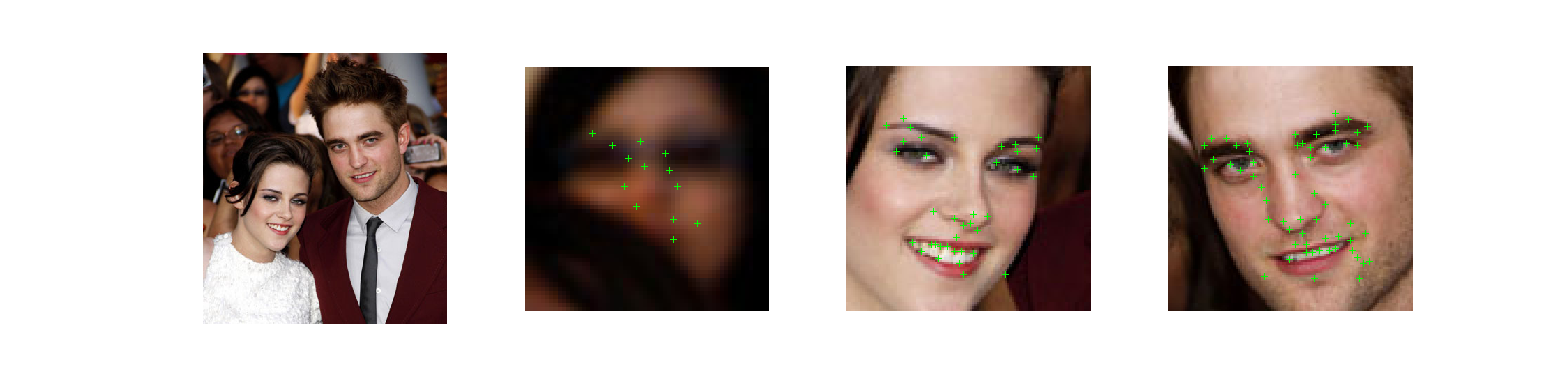
\includegraphics[width=0.7\linewidth]{figures/corner_detection.png}
\caption{corner detection on each face detected in the test image}
\end{figure}

\begin{figure}[h!]
\centering
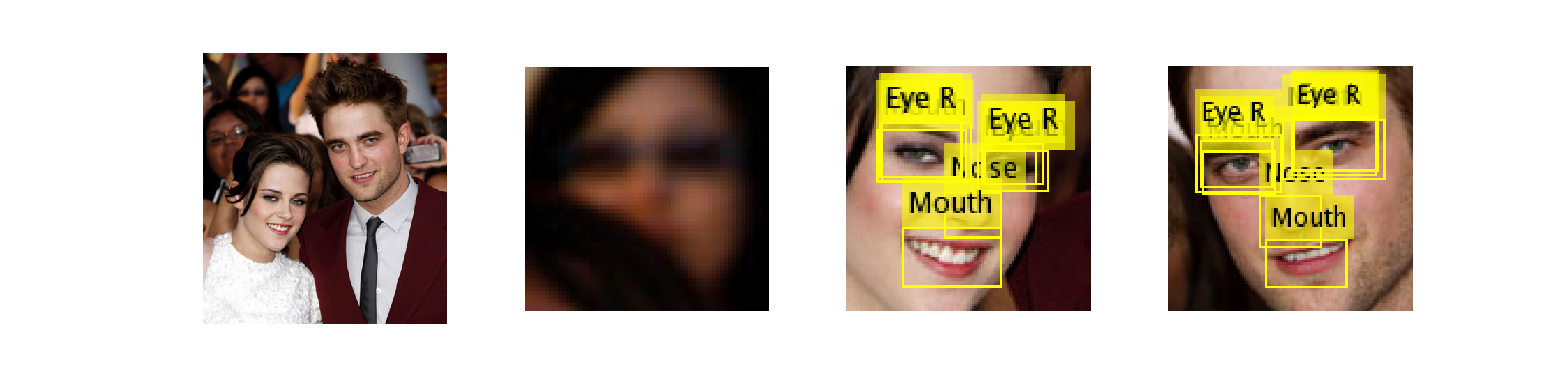
\includegraphics[width=0.7\linewidth]{figures/component_detection.png}
\caption{detecting face components on each face detected in the test image}
\end{figure}

\end{document}